\clearpage
\section{IAD解析}

\begin{figure}[H]
  \centering
  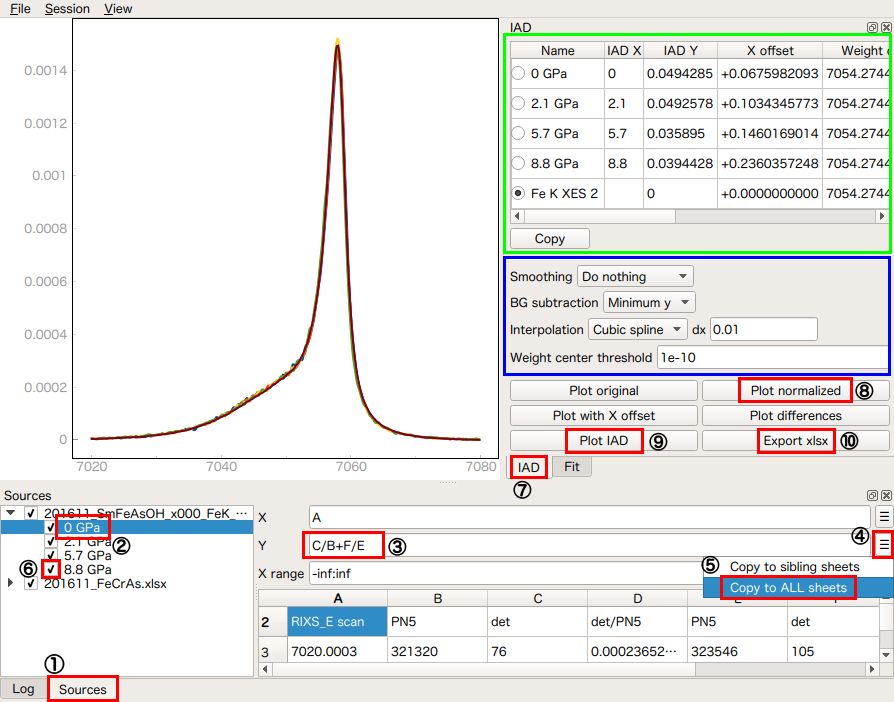
\includegraphics[width=10cm]{images/IAD-1.png}
  \caption{IAD解析画面}
  \label{fig:IAD-1}
\end{figure}

\subsection{基本的な手順}

\begin{enumerate}
\item 測定データの入ったファイルをTunaのウィンドウにドラッグ\&ドロップして開く.
  複数のファイルを同時にドラッグしたり, 連続して開いたりできる.
  テキストファイル, CSV, MS Excel, LibreOffice等のフォーマットに対応している.
\item 左下の\kwR{Sources}タブ(\cnum{1})をクリックする.
\item 左下のツリービューで, 適当なシートを選択する(\cnum{2}).
  図\ref{fig:IAD-1}は2つのエクセルファイルを開いた場合の画面である.
\item 読み込むべきスペクトルの $x$, $y$ 座標にあたる列を右下の\kwR{X}, \kwR{Y}の欄(\cnum{3})に記入する.
  \kwR{X}, \kwR{Y}はいずれも任意の数式を記入できる.
  また1シートに複数のスペクトルが記録されている場合, カンマ(,)で区切って複数の数式を記入できる.
\item 他のシートも同様に\kwR{X}, \kwR{Y}を記入する. すべてのシートに同じ式を使う場合,
  右端のメニューボタン(\cnum{4})を押してメニューから\kwR{Copy to ALL sheets}(\cnum{5})%
  を選択すると全シートにコピーされる.
\item 全シートに式を記入したら, 適当なシートのチェックを外し, チェックし直す(\cnum{6}).
  これで式の再読み込みが行われる. また, 使わないシートはチェックを外しておく.
\item 右上ペイン下部の\kwR{IAD}タブ(\cnum{7})をクリックする.
\item \kwR{Plot normalized}ボタン(\cnum{8})をクリックしてスペクトルが正しく読み込まれていることを確認する.
\item \kwR{Plot IAD}ボタン(\cnum{9})をクリックして結果を確認する.
\item 必要なら, \kwR{Export xlsx}ボタン(\cnum{10})で検算用のエクセルファイルを書き出す.
\end{enumerate}

\subsection{UI各部の説明}

\begin{itemize}
\item \kwG{右上テーブル} 解析結果を表示する. 選択範囲をエクセル等にコピーペーストできる.
  \begin{itemize}
  \item \kwG{Name} 各スペクトルの名前. 読み込んだファイル名またはシート名をもとに作成される.
    ラジオボタンで基準スペクトルを選択する. 基準スペクトルのIAD値は必ず $0$ となる.
  \item \kwG{IAD X} IAD値をプロットする際の横軸の値. 例えば圧力変化を測ったなら, 圧力値を入力する.
  \item \kwG{IAD Y} IAD値の計算結果.
  \item \kwG{X offset} 重心を合わせるために横シフトした量.
  \item \kwG{Weight center} 重心の値.
  \item \kwG{Peak x} ピーク位置 $x$ 座標.
  \item \kwG{Peak y} ピーク位置 $y$ 座標.
  \end{itemize}
\item \kwG{Copy} テーブルの内容をすべてコピーする. エクセル等にペーストできる.
\end{itemize}

\vspace{1em}

\begin{itemize}
\item \kwB{Smoothing} スムージングの方法を指定する. 現在, Savitzky-Golayフィルタ%
  (\scipy{scipy.signal.savgol\_filter})のみ実装している.
\item \kwB{BG subtraction} バックグラウンド除去の方法を指定する.
  \begin{itemize}
  \item \kwB{Minimum y} スペクトルの最小値をバックグラウンドとして定数引く.
  \item \kwB{Left edge} スペクトルの左端から \kwB{deltaX} の範囲で平均値をとり,
    これをバックグラウンドとして定数引く.
  \item \kwB{Right edge} スペクトルの右端から \kwB{deltaX} の範囲で平均値をとり,
    これをバックグラウンドとして定数引く.
  \end{itemize}
\end{itemize}

\vspace{1em}

\begin{itemize}
\item \kwB{interpolation} 内挿の方法を指定する.
\item \kwB{dX} 内挿の間隔を指定する.
  \begin{itemize}
  \item \kwB{Cubic spline} \texttt{\scipy{scipy.interpolate.CubicSpline}(x, y)}
  \item \kwB{B-spline} \texttt{tck=\scipy{scipy.interpolate.splrep}(x, y, w)},
    \texttt{\scipy{scipy.interpolate.splev}(x, tck)}
    \kwB{w} には \code{x}, \code{y}, \code{ymax} を変数とした任意の式を記入できる.
    測定値の誤差が $d$ で与えられる場合, $w=1/d$ とする.
    ピークの高いところは測定値に合わせるが, 低いところはスムーズにしたい場合,
    例えば \code{w=1/(ymax*0.003*(1.00001-y/ymax))} 等とすると良い.
  \item \kwB{Linear} \texttt{\scipy{scipy.interpolate.interp1d}(x, y, "linear")}
  \item \kwB{Pchip} \texttt{\scipy{scipy.interpolate.PchipInterpolator}(x, y)}
  \item \kwB{Akima} \texttt{\scipy{scipy.interpolate.Akima1DInterpolator}(x, y)}
  \item \kwB{Krogh} \texttt{\scipy{scipy.interpolate.KroghInterpolator}(x, y)}
  \item \kwB{Barycentric} \texttt{\scipy{scipy.interpolate.BarycentricInterpolator}(x, y)}
  \end{itemize}
\item \kwB{Weight center threshold} 各スペクトルと基準スペクトルの重心の差がこの値より小さくなるよう,
  \kwG{X offset} を調整する. 例えば $1$ 等じゅうぶん大きな値に設定しておくと,
  スペクトルの横シフトを行わずにIAD値を計算する.
\end{itemize}

\vspace{1em}

\begin{itemize}
\item \kwR{Plot original} 各シートの \kwR{Y} 欄に記入した式の評価結果(生の測定値)をそのままプロットする.
\item \kwR{Plot normalized} 各スペクトルに対し, スムージング, バックグラウンド除去, 内挿を行ったあと,
  $\sum y_i = 1$ となるようノーマライズしてプロットする.
\item \kwR{Plot with X offset} 各スペクトルに対し \kwR{Plot normalized} と同じ手続を行ったあと,
  重心のばらつきが \kwB{Weight center threshold} より小さくなるよう横方向にずらしてプロットする.
\item \kwR{Plot differences} 各スペクトルに対し \kwR{Plot with X offset} と同じ手続を行ったあと,
  基準スペクトルとの差をプロットする.
\item \kwR{Plot IAD} 各スペクトルに対し \kwR{Plot with X offset} と同じ手続を行ったあと,
  IAD値を計算し, \kwG{IAD X} とあわせてプロットする.
\item \kwR{Export xlsx} 検算用のエクセルファイルを書き出す.
\end{itemize}
